\newpage
\subsection{Map subsystems to processors and components}
\begin{figure}[htb!]
    \centering
    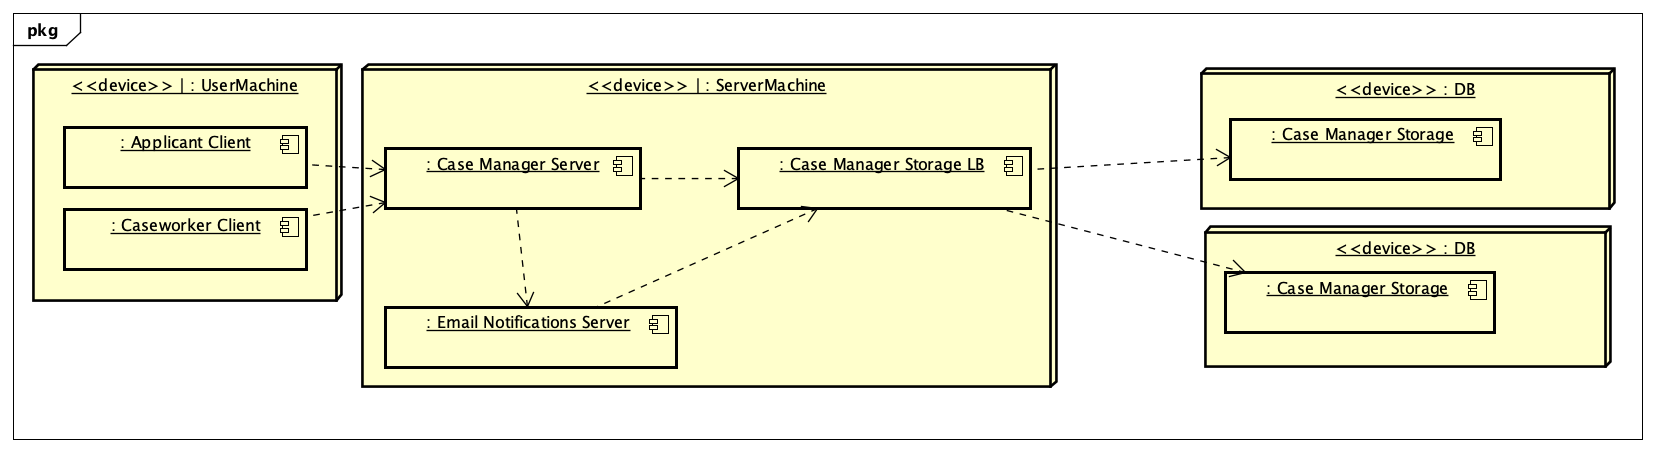
\includegraphics[width=\textwidth]{img/pkg-deployment-diagram.png}
    \caption{Deployment Diagram}
\end{figure}

We have chosen to have a separate email notification server, that would handle a queue of outgoing notifications and handles these notifications in an interval.
Second, we have a load balancing system that will handle incoming requests and distribute them out of the available storage servers. 
The persistent storage should support replication (like MySQL replication) to ensure data reliability.
With this setup, we possibly suffer some performance, but that should be dealt with by including an efficient cache setup on the load balancing server. Other than that, when we have actually persistence, we would do that asynchronously, so the delay would be kept to a minimal.